% -*- TeX:de -*-
\NeedsTeXFormat{LaTeX2e}
\documentclass[12pt,a4paper]{article}
\usepackage[english]{babel} % german text
\usepackage[DIV12]{typearea} % size of printable area
\usepackage[T1]{fontenc} % font encoding
%\usepackage[latin1]{inputenc} % most likely on Windows
\usepackage[utf8]{inputenc} % probably on Linux
\usepackage{multicol}
% PLOTTING
\usepackage{pgfplots}
\usepackage{pgfplotstable}
\usepackage{url}
\usepackage{graphicx} % to include images
\usepackage{tikz}
\usepackage{subfigure} % for creating subfigures
\usepackage{amsmath} % a bunch of symbols
\usepackage{amssymb} % even more symbols
\usepackage{booktabs} % pretty tables
\usepackage{makecell} % multi row table heading
% a floating environment for circuits
\usepackage{float}
\usepackage{caption}
\usepackage{hyperref}
\usepackage{eurosym}

% Title Page command
\newcommand{\HRule}{\rule{\linewidth}{0.5mm}}

%\newfloat{circuit}{tbph}{circuits}
%\floatname{circuit}{Schaltplan}
% a floating environment for diagrams
%\newfloat{diagram}{tbph}{diagrams}
%\floatname{diagram}{Diagramm}
\pgfplotsset{compat=1.8}
\selectlanguage{english} % use german
\begin{document}
%%%%%%% DECKBLATT %%%%%%%
\begin{titlepage}
\begin{center}

% Upper part of the page. The '~' is needed because \\
% only works if a paragraph has started.

\includegraphics[scale=0.75]{./unilogo}~\\[2cm]

\textsc{\LARGE University of Vienna }\\[0.5cm]
\textsc{\LARGE Faculty of Physics}\\[1.5cm]
\textsc{\Large Quantum optics practical course}\\[0.5cm]

% Title
\HRule \\[0.4cm]
{ \huge \bfseries Radiaton Pressure}\\[0.4cm]

\HRule \\[1.5cm]

% Author and supervisor
\begin{minipage}{0.4\textwidth}
\begin{flushleft} \large
\emph{Author:}\\
Johannes \textsc{Kurz}\\
\emph{Group:}\\
\textsc{Braun, Donabaum, Kurz}\\
\end{flushleft}
\end{minipage}
\begin{minipage}{0.4\textwidth}
\begin{flushright} \large
\emph{Supervisor:} \\
Witlef \textsc{Wieczorek}
\end{flushright}
\end{minipage}

\vfill

% Bottom of the page
{\large 31.10.2014}

\end{center}
\end{titlepage}
%%%%%%% DECKBLATT ENDE %%%%%%%
\pagebreak
\setlength{\columnsep}{20pt}
\begin{multicols}{2}

\begin{abstract}

\end{abstract}

%%%%%%%%%%%%%%%%%%%%%%%%%%%%%%%%%%%%%%%%%%%%%%%%
%\begin{figure}[H]
% \centering
% \includegraphics[scale=0.35]{./data/beugung.png}
% \caption{Beugungsmuster Einzelspalt (echtes Foto; schwarz durch weiß ersetzt)}
% \label{fig:beugungsmuster}
%\end{figure}
%\begin{figure}[H]
% \centering
% \pgfplotstabletypeset[
% columns={abstand, n},
% col sep=&,
% columns/abstand/.style={precision=2, zerofill, column name=\makecell{$Abstand$\\$(\pm 0.05)[mm]$} },
% columns/n/.style={column name=\makecell{$n$\\$(Ordnung)$}, precision=0},
% every head row/.style={before row=\hline,after row=\hline\hline},
% every last row/.style={after row=\hline},
% every first column/.style={column type/.add={|}{} },
% every last column/.style={column type/.add={}{|} }
% ]{
% abstand & n
% 12.9 & 1
% 24.45 & 2
% 37.40 & 3
% 49.35& 4
% 62.45 & 5
% 74.45 & 6
% 87.45 & 7
% 100.25 & 8
%
% }
% \caption{Messwerte Einzelspalt}
% \label{tab:werte_einzelspalt}
%\end{figure}
%%%%%%%%%%%%%%%%%%%%%%%%%%%%%%%%%%%%%%%%%%%%%%%%
%%%%%%%%%%%%%%%%%%%%%%%%%%%%%%%%%%%%%%%%%%%%%%%%

\section{Bell's Inequality}
This work is intended to show that entanglement cannot be described in a classical way. It was the work of J.S. Bell based on the paper of Einstein, Podolsky and Rosen (EPR). With the CHSH-Bell inequality it became possible to do a (rather) simple experiment with photons. In the next sections the theory will be explained as well as the experimental assembly and the results. Finally we will discuss the outcome.

%%%%%%%%%%%%%%%%%%%%%%%%%%%%%%%%%%%%%%%%%%%%%%%%
%%%%%%%%%%%%%%%%%%%%%%%%%%%%%%%%%%%%%%%%%%%%%%%%
\section{Theory}
\label{theory}

\subsection{Entanglement}

\subsection{CHSH-Bell Inequallity}

\subsection{Loopholes}

\subsection{Birefringence}

\subsection{Two-photon coincidence fringe visibility}

\subsection{CHSH-Bell parameter}

%%%%%%%%%%%%%%%%%%%%%%%%%%%%%%%%%%%%%%%%%%%%%%%%
%%%%%%%%%%%%%%%%%%%%%%%%%%%%%%%%%%%%%%%%%%%%%%%%
\section{Experimental assembly}

\subsection{Build}

\subsection{Alignment}

\begin{figure}[H]
 \centering
 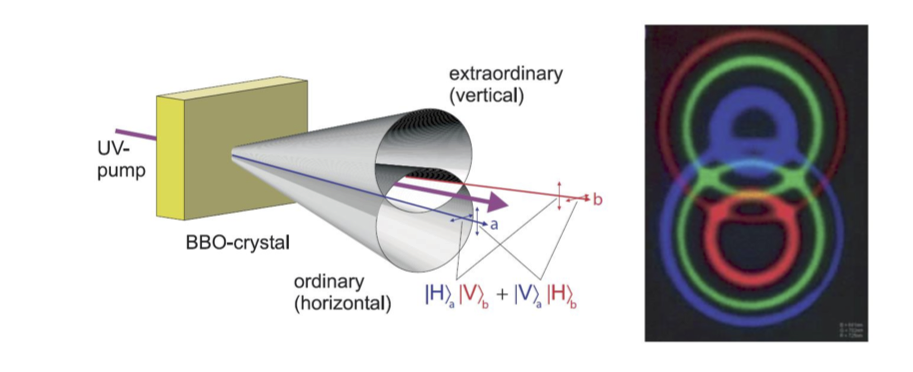
\includegraphics[scale=0.7]{./figures/cones.png}
 \caption{Cones created after the BBO \cite{physikwiki}[p. 9]}
 \label{fig:cones}
\end{figure}

\subsubsection{BBO}
\subsubsection{Waveplates}
\subsubsection{Prismas}
\subsubsection{Stages, Fibers and Detectors}

%%%%%%%%%%%%%%%%%%%%%%%%%%%%%%%%%%%%%%%%%%%%%%%%
%%%%%%%%%%%%%%%%%%%%%%%%%%%%%%%%%%%%%%%%%%%%%%%%
\section{Results}
The full document and the results contained in a QTI file and a Excel sheet can be found under \cite{github}
\subsection{visibility}
requirement: $vis > \frac{1}{\sqrt{2}} = 0.707$
\noindent \textbf{H/V - Basis:}\\

%\begin{figure}[H]
% \centering
% \pgfplotstabletypeset[
% columns={what, value},
% col sep=&,
% columns/what/.style={column name=\makecell{$Measurement$}, string type},
% columns/value/.style={column name=\makecell{$Coincidences$}, precision=0, zerofill},
% every head row/.style={before row=\hline,after row=\hline\hline},
% every last row/.style={after row=\hline},
% every first column/.style={column type/.add={|}{} },
% every last column/.style={column type/.add={}{|} }
% ]{
% what & value
%$AH, BH$ & 3
%$AH, BV$ & 55
%$AH, BH-$ & 5
%$AH, BV- $& 55
%$AV, BH$ & 69
%$AV, BV$ & 1
%$AV, BH- $& 70
%$AV, BV-$ & 1
%
% }
% \caption{Messwerte Einzelspalt}
% \label{tab:werte_einzelspalt}
%\end{figure}

$Vis_{HV}= (0.918 \pm 0.047) > \frac{1}{\sqrt{2}}$\\
\\
\textbf{X$^+$/X$^-$ - Basis before optimization}\\

$Vis_{X^+ X^- before}=(0.650 \pm 0.087) < \frac{1}{\sqrt{2}}$\\
\\
\textbf{X$^+$/X$^-$ - Basis}\\

$Vis_{X^+ X^- }=(0.843 \pm 0.032) > \frac{1}{\sqrt{2}}$\\

\subsection{Bell-measurements}




%%%%%%%%%%%%%%%%%%%%%%%%%%%%%%%%%%%%%%%%%%%%%%%%
%%%%%%%%%%%%%%%%%%%%%%%%%%%%%%%%%%%%%%%%%%%%%%%%
\section{Discussion}


%%%%%%%%%%%%%%%%%%%%%%%%%%%%%%%%%%%%%%%%%%%%%%%%
%%%%%%%%%%%%%%%%%%%%%%%%%%%%%%%%%%%%%%%%%%%%%%%%

\bibliography{protocol.bib}
\bibliographystyle{plain}

\end{multicols}
\end{document}